\documentclass[colorback,accentcolor=tud1c,11pt]{tudreport}
\usepackage[english]{babel}
\usepackage[utf8x]{inputenc}
%\usepackage[T1]{fontenc}

%\usepackage[stable]{footmisc}
%\usepackage[ngerman,pdfview=FitH,pdfstartview=FitV]{hyperref}

\usepackage{booktabs}
%\usepackage{multirow}
%\usepackage{longtable}
\usepackage{listings}
\usepackage{graphicx}
\usepackage{subfigure} 	
\usepackage{float}
\usepackage{amsmath}

\newcommand\todo[1]{\textcolor{red}{#1}}
\newcommand\code[1]{\texttt{#1}}
%\usepackage{floatflt}

\graphicspath{{./img/}}

%\newlength{\longtablewidth}
%\setlength{\longtablewidth}{0.675\linewidth}

\title{Mini-task report: Espresso Logic Minimization}
\subtitle{Mitja Stachowiak, Ludwig Meysel}

\begin{document}
  \maketitle

  \chapter{Introduction}

  The task was to implement a simple verino of the logic minimization algorithm ESPRESSO. Given are non-hierarchical BLIF files which can define one or more output variables. There must be found a efficient encoding for a positional cube notation. After running ESPRESSO on the boolean function the minimized function should be written again as a BILF file.

  \chapter{BLIF Parser}

  For the Minitasks a BLIF parser for finite state machines is given. A short analysis of the given parser makes it easy to implement the own parser for the simpler BLIF data. There is no need to consider any status information, but just the input combinations and the outputs for them. Fig.~\ref{fig:egblif1} shows a simple example of a boolean function defined in BLIF. The function consists only of an ON-set, the DC-set is neglegted at this point.

  \begin{figure}
	  \centering
	  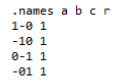
\includegraphics{img-blif}
	  \caption{Example for a BLIF defined boolean function}
	  \label{fig:egblif1}
  \end{figure}

  Starting with a filename given to a parser-method the parser creates a \code{Model} object which then contains a list of \code{BinFunction}s with their named inputs and outputs. Fig.~\ref{fig:egblif1} shows just one boolean function, but a BLIF file could contain multiple of them. It can even refer to other BLIF files. Therefore the \code{Model}-object contains a list of \code{BinFunction}s.
  \\
  The parser reads the input variables and encodes them in positional cube notation in Java's \code{long} primitive. In the positional cube notation each boolean varible is encoded with two bits. A \code{long} has 64 bits and can therefore handle 32 boolean variables in positional cube noation, within one long-variable. To be able to handle more than 32 boolean variables, a \code{Cube}-object handles a \code{long}-Array which makes it theoretically possible to handle arbitrary numbers of boolean variables. Actually there are other (physical) limits for the number of boolean variables, which at least are made up with the size of the internal memory.
  \\
  Espresso must be able to handle nearly each posible input combination in one \code{BinFunction}. When there are 32 input varbiables for one function, there are nearly $2^{32}$ possible input combinations, each taking one \code{long}-value. Therefore the required memory for a 32-input-\code{BinFunction} would be up to $2^{32} \times 4 Byte \sim 16 GB$! This space requirement doubles which each more input variable. It is therefore a discussion point whether it makes sense to implement a cube with a \code{long}-array or just set a limit in our implementation by using just one \code{long}. On the one hand it is nice to have an algorithm which is not limited by its implementation. On the other hand using just one \code{long}-value avoids the necessity of calculating the array-offset when checking one specific variable, which could save time because it avoids many divisions. In our implementation we decided for the first approach, using the \code{long}-array.
  

  \chapter{Implementation of Espresso}
  Espresso runs mainly in two phases \cite{micheli2003synthesis}:
  \begin{itemize}
  	\item{compute the complement}
	\begin{item}
		Iterate until cost function not further shrinks
		\begin{itemize}
			\item{expand}
			\item{remove irredundant cubes}
			\item{reduce}
		\end{itemize}
	\end{item}
  \end{itemize}

  \section{Computation of the complement}
  We decided to spare the computation of the function complement - there are more or less easy-to-implement approaches which handle different problems coming up with the computation. One of the main challenges of the complement computation is as already mentioned before: Memory. Having a 32-input-\code{BinFunction} would at least now lead to a memory-problem if the complement cannot be computed directly optimized.
  \par
  A straight-forward approach would be to iterate over each combination of the function and remove all those which are already included in the ON-set or the DC-set. But using a 32-input-function again would result in a huge amount of implicants, which require a lot of memory. Additionally, checking the expanded cubes against the non-optimized OFF-set results in very much iterations. So it is obvious that calculating the complement does only make sense when getting a more or less simplified result. The function BinFunction.computeOff() processes DeMorgan's law over the complete function. The bottleneck here is the multiplication of all KNF-terms. Even if invalid multiplication-paths like a * a' are skipped, this function quickly runs out of memory, even for function having less than 10 variables. There exist better approaches for complementation, but this task was more about implementing espresso therefore we decided to spare the computation of the OFF-set and used the PRESTO-approach, which checks for each Expansion, not if it intersects with the OFF-set but if it's still covered by the ON+DC-set before the expansion. The functions for checking, if a cube is completely covered by a set, are required for the reduction-phase anyway. But a basically similar algorithm can also be used, to compute an intersect-free set in the beginning of Espresso. With an intersect-free set, the covering-check can be done mach more efficient by summing the cardinalities of the intersection-sets between the set's cubes and the cube to be tested against the set. While the intersect-test against the OFF-set can stop as soon as it finds the first intersection, the covering-test against the ON+DC-set has to process all cubes of the set and has some overhead with computing cardinalities (counting DCs) and doing the summation.
  \par
  According to the lecture, it is already known, that ESPRESSO in general would run faster with the initial complement computation instead of using the PRESTO approach. We decided to use the PRESTO approach, however, to focus on the ESPRESSO implementation itself, but not on the complement computation.

 \section{Expansion}
 The expansion tries to create greater cubes, i. e. cubes which cover more minterms. Therefore an expanded cube has covers at least two minterms. The second expansion would cover four minterms, and so on. All of those minterms must be part of the ON- or DC-set, but must not be part of the OFF-set. As already mentioned in our implementation there is no explicit knowledge about the OFF-set, therefore each expanded cube must be part of the ON- or DC-set.

 \section{Remove redundant cubes}
 The removal of redundant cubes offers some new interesting issues. Fig.~\ref{fig:redundancy} (a) shows 5 possible cubes. First, there are different combinations which result in possible sets. Obviously (c) is better than (b) due to the fact that it has no redundancy. How to remove redundant cubes has already been explained within the lecture \cite{Hochberger2017}, and therefore wont be descussed here.
 \begin{figure}
   \centering
   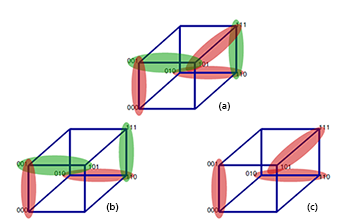
\includegraphics{redundancy}
   \caption{Possible cubes (a), redundand cubes (b), optimal set (c); Source: \cite{Hochberger2017}}
   \label{fig:redundancy}
 \end{figure}

 A more interesting problem at this point is, how to handle irredundant cubes. As depicted in fig.~\ref{fig:redundancy} (b) there are four cubes which intersect and obviously there could be found a better set (c). The problem here is, that in this constellation all cubes are essential, and therefore they are removed from the ``working''-set, the one which will be reduced in the next step. But when removing all four essentials from the working-set, it is empty then and the algorithm terminates.
 \par
 On the one hand this is a result of the heuristic approach, on the other hand, it looks like this a problem which could be solved easily. When having a closer look to the function (see fig.~\ref{fig:redundancy2}) and inspecting the column- and row-sums of the function, we see there will happen no reordering of the minterms, whereas this reordering is fundamental for the heuristic. One approach would be, to reorder the rows randomly when the row-sums are equal. But minimizing the function this way, in the worst case every possible combination must be tried in order to minimize the original function. For larger functions that could take a very long time. Therefore it is reasonable to neglect this very special and unlikely case.

 \begin{figure}
   \centering
   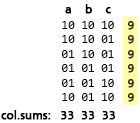
\includegraphics{redundancy2}
   \caption{Column- and row-sums of function in fig.~\ref{fig:redundancy}}
   \label{fig:redundancy2}
 \end{figure}

 \section{Reduction}
 The reduction is kind of the reverse operation of the expansion. Dont-cares are tried to set to zero or ones. This change is accepted when the whole function is still covered.

 \chapter{Evaluation}
 For the evaluation some benchmarks have been tested. The main focus is on the runtime of the algorithm, the number of cubes before and after the minimization. As reference the \textit{ABC Sequential Systhesis and Verification} package is given for comparing the results. First of all, the runtime of the ABC-implementation is not really comparable to ours. What ABC does within a ``tick'' takes multiple minutes in our implementation of ESPRESSO. For smaller examples our implementation works fine when the following condiditions are given:
 \begin{itemize}
  \begin{item}
  No dont-care-outputs should exist. The problem with dont-cares is not that our algorithm does not work, but it seems ABC ignores these dont-cares. Therefore our results could not be validated reliably. A specific test was the benchmark \textit{hard\_examples/pdc}. This file is completely separated in ON-set and DC-set. When removing the DC-set, our implementation seems to return an equal result like ABC (i.e. same number of cubes and random samples were equal). Keeping the DC-set our implementation reduces the number of cubes drastically, whereas ABC seems to ignore the DC-set.
  \end{item}
  \begin{item}
  Our solution seems to have a bug which we could not fix due to the remaining time for the minitask. It seems to be an issue with the calculation of the \code{long}-array-offset for functions with more than 32 Variables. At this point there are at least two longs per cube required. The offset seems to be calculated wrong at any point.
  \end{item}
\\
  For those functions where our implementation seems to work correctly was the minimization as depicted in table~\ref{tbl:foobar}.

  \begin{table}
    \center
    \begin{tabular} { | l | c | c | c | c | c |}
      \hline
      \textbf{Benchmark} & inputs & functions &  cubes total & cubes ABC &  cubes our impl. \\
      \hline
      lion\_Binary.blif (Moodle-Example) & 4 & 3 & 18 & 11 & 11 \\
      pdc (DCs removed) & 16 & 40 & 2417 & 448 & 449 \\
      ex1010 (setting DCs to ON) & 10 & 10 & 1146 & 1026 & 1090 \\
      ex1010 & 10 & 10 & 1026 & 953 & 465 \\
      \hline
    \end{tabular}
    \caption{Results comparison}
    \label{tbl:foobar}
  \end{table}

 \end{itemize}
 
 \chapter{Conclusion}
 Espresso turned out to be a very broad resarch field. There are many possibilities a developer can optimize the algorithm. The main problem we were not able to solve is the calculation of the OFF-set which is, according to the lecture, probably one of the biggest performance losses. Therefore the next step to continue this project would be to find an efficient computation of the complement of a set. Another pretty important To-Do is the bugfixing for functions having more than 32 variables.
 \\
  The project is realized in about 2300 lines of code.

  \bibliographystyle{plain}
  \bibliography{references}
\end{document}

